\section{Results}

\subsection{Stability of Hopfield Network}
\begin{figure}[H]
    \centering
    \begin{subfigure}{0.49\textwidth}
        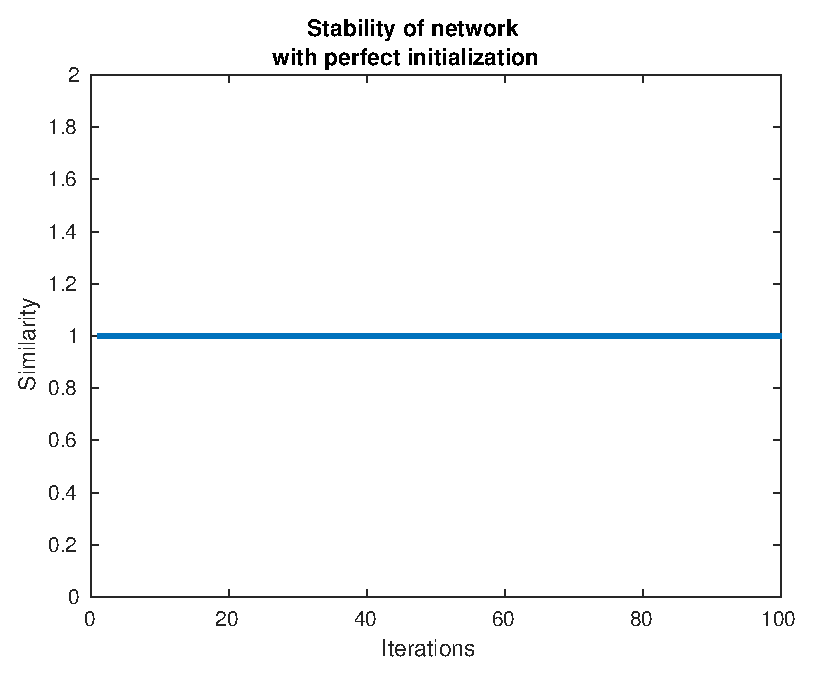
\includegraphics[width=\textwidth]{figs/stable}
        \caption{By initializing the network to the stored pattern, the network will remain in an equilibrium. The network will never deviate from this state without external interference.}
    \end{subfigure}
    \begin{subfigure}{0.49\textwidth}
        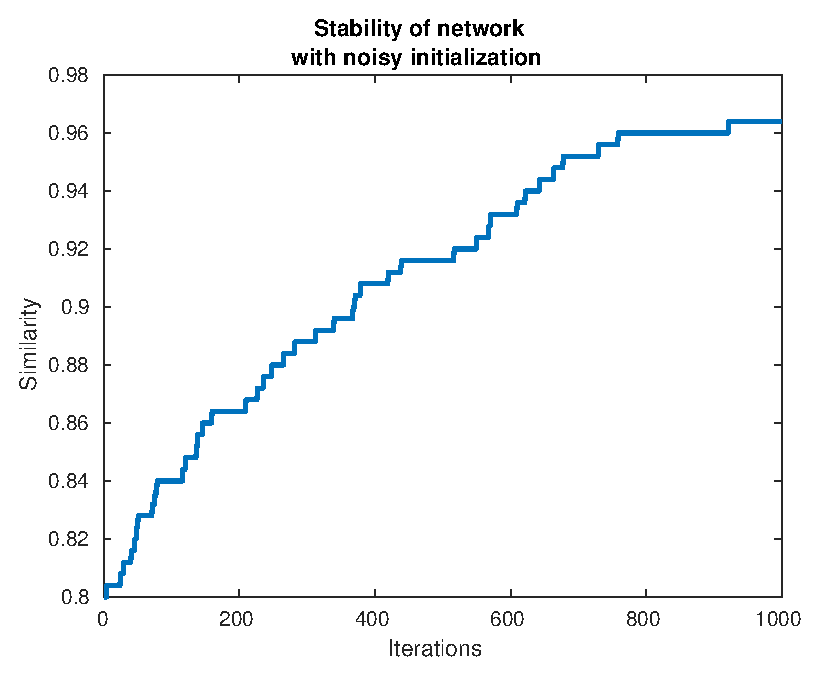
\includegraphics[width=\textwidth]{figs/stable-with-noise}
        \caption{If the network is initialized to a noisy state, the network will converge towards the stored pattern. }
    \end{subfigure}
    \caption{Initializing a Hopfield network with a single stored pattern will cause the network to converge towards the stored pattern.}
\end{figure}

\subsection{Storing multiple patterns}
\begin{figure}[H]
    \centering
    \begin{subfigure}{0.49\textwidth}
        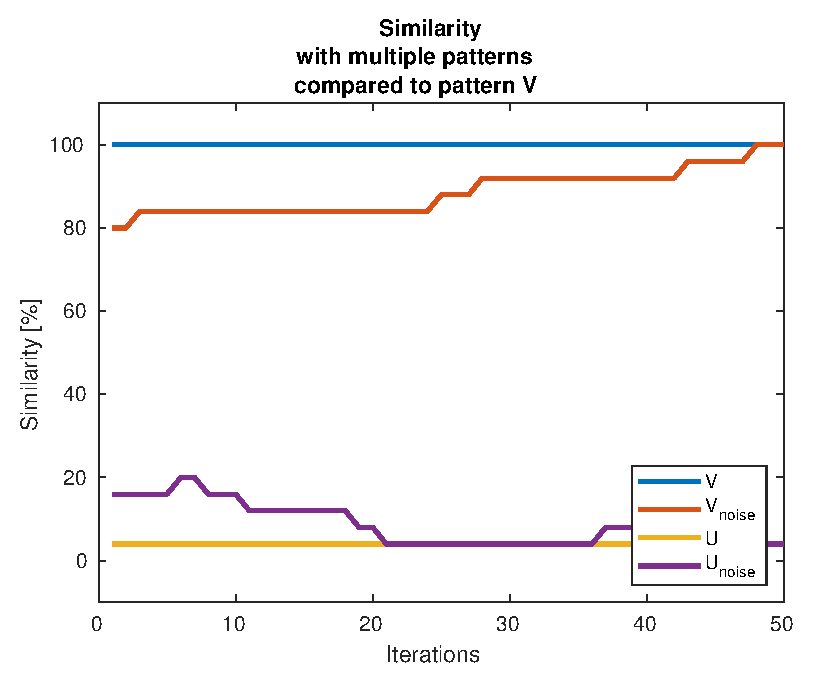
\includegraphics[width=\textwidth]{figs/multiple-patterns.eps}
        \caption{By initializing the weight matrix $\bf W$ with multiple patterns, the network is able to restore multiple different patterns. The amount of memories and noise the network is able to handle, depends on complex the pattern is (number of neurons) and how similar the patterns are. If two stored patterns only differ by one bit, the network may recall the wrong memory if noise is involved. }
    \end{subfigure}
    \begin{subfigure}{0.49\textwidth}
        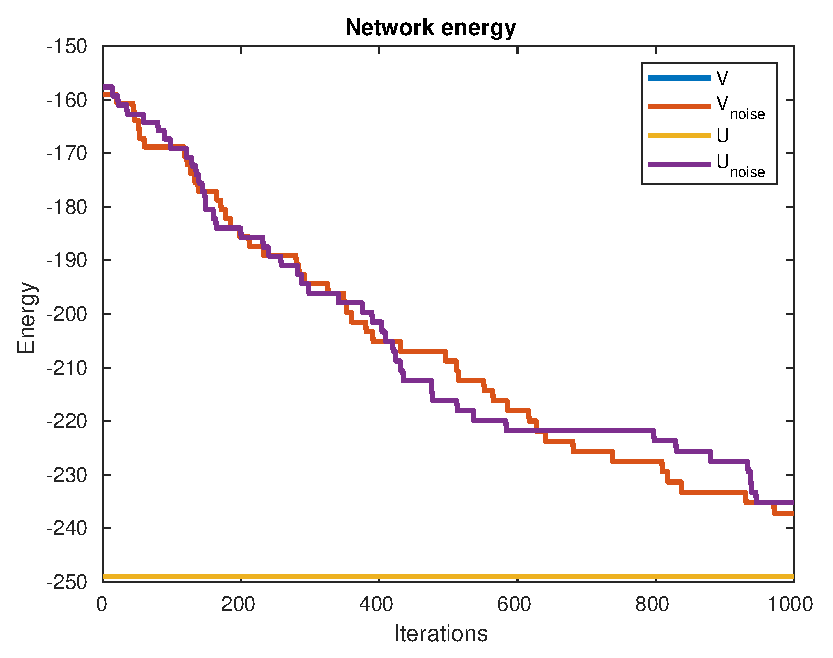
\includegraphics[width=\textwidth]{figs/multiple-patterns-energy.eps}
        \caption{The network will always move in the direction of least resistance such that the overall energy decrease, similar to how a ball always will roll downwards into a valley unless there are external forces interfering. Each stored memory corresponds to a local minimum which can be thought of as valleys, and as long as the network is initialized in the correct valley, it is able to reconstruct the state from memory.}
    \end{subfigure}
\end{figure}
 

\subsection{Reconstructing partially lost QR codes from memory}
\begin{figure}[H]
    \centering
    \begin{subfigure}{0.49\textwidth}
        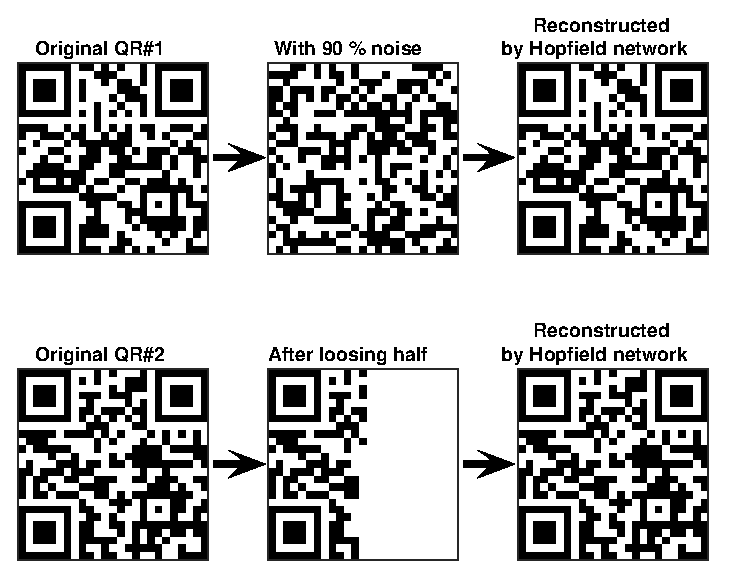
\includegraphics[width=\textwidth]{figs/qr-code}
        \caption{The QR-code contains information encoded within the patterns. A QR decoding app, either online or on a smartphone, can be used to decode the "hidden" message. Using the hopfield network we are able to reconstruct a destroyed QR-code from memory.}
    \end{subfigure}
    \begin{subfigure}{0.49\textwidth}
        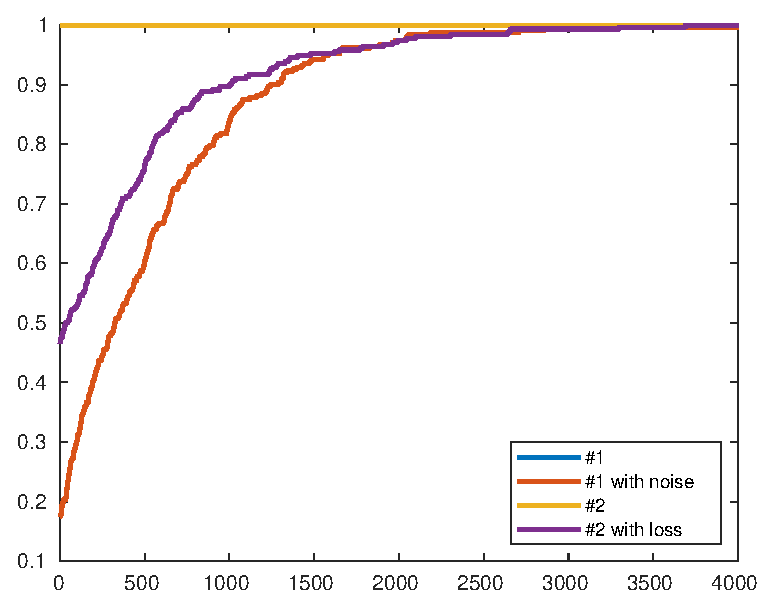
\includegraphics[width=\textwidth]{figs/qr-code-sim}
        \caption{The similarity between the current state of the network and the original QR-code.}
    \end{subfigure}
    \caption{By applying the Hopfield network to a very noisy QR-code we are able to reconstruct the original. By using any QR-code reader we are able to decode the left and right QR-codes, while the middle ones contains too much noise. The same hopfield network was used. The QR-code patterns were stored in addition to a third random pattern. }
\end{figure}